\chapter{Grundlagen}

\section{Bestehende Technologien und Hardware:}

\subsection{Funktionsweise eines KaVo Behandlungsstuhls}

\subsubsection{Allgemeine Funktionen und Zweck}

Ein moderner Behandlungseinheit ist das zentrale Element jeder Zahnarztpraxis. Er dient nicht nur als ergonomische Sitz- und Liegeeinheit für den Patienten, sondern integriert alle notwendigen Instrumente, Steuer- und Versorgungseinheiten in einer kompakten Arbeitsumgebung. Der Behandler kann Position, Beleuchtung und Instrumentenzugriff flexibel anpassen, um eine präzise und effiziente Behandlung zu gewährleisten.


\subsubsection{Technische Architektur und Steuerung}

\paragraph{Controller Area Network (CAN-Bus):}

\leavevmode

Das \textit{Controller Area Network (CAN)-Bus} ist ein standardisiertes serielles Bussystem, das ursprünglich für die Kommunikation zwischen Steuergeräten in der Automobiltechnik entwickelt wurde. Es ermöglicht, mehrere elektronische Steuerplatinen über ein einziges, robustes Leitungsnetzwerk zu verbinden, ohne dass aufwendige Punkt-zu-Punkt-Verkabelungen notwendig sind.

Im KaVo-Behandlungsstuhl dient der CAN-Bus als zentrales Kommunikationsmedium: Alle Funktionseinheiten — wie die Stuhlpositionssteuerplatine, die Lichtsteuerplatine, die Instrumentensteuerplatine sowie die Bildverarbeitungs- und Netzwerkkomponenten — tauschen Steuerbefehle, Sensordaten und Statusinformationen zuverlässig über dieses Netzwerk aus.

Die Kommunikation erfolgt nach dem Broadcast-Prinzip: Jede Nachricht wird an alle Teilnehmer gesendet, wobei jedes Steuergerät anhand einer eindeutigen ID prüft, ob die Information für seinen eigenen Aufgabenbereich relevant ist. So können Steuerungen modular hinzugefügt oder ausgetauscht werden, ohne die gesamte Systemarchitektur zu verändern.

Die Signalübertragung erfolgt differenziell über verdrillte Adernpaare. Ein \textbf{dominantes Bit} (logisch „0“) wird durch einen definierten Spannungsunterschied zwischen \textit{CAN High} und \textit{CAN Low} erzeugt, während bei gleichem Pegel ein \textbf{rezessives Bit} (logisch „1“) übertragen wird. Diese Technik macht den CAN-Bus besonders widerstandsfähig gegenüber elektromagnetischen Störungen — ein entscheidender Vorteil in einer Praxisumgebung mit zahlreichen elektrischen Geräten.

Ein zentrales Merkmal des CAN-Bus ist die konfliktfreie Kommunikation über die sogenannte \textit{Arbitration}: Beginnen mehrere Knoten gleichzeitig mit einer Übertragung, vergleichen sie während der Übertragung der ID-Bits kontinuierlich den gesendeten Pegel mit dem aktuellen Buspegel. Erkennt ein Knoten, dass er ein rezessives Bit gesendet hat, der Bus jedoch dominant ist, so erkennt er eine höhere Priorität eines anderen Knotens und bricht die eigene Übertragung sofort ab. Nur der Knoten mit der höchsten Priorität setzt die Übertragung fort; alle anderen warten, bis der Bus wieder frei ist.

\paragraph{KaVo Behandlungsthul Steuerplatinen-Topologie:}

\leavevmode

Die Steuerung eines KaVo-Behandlungsstuhls basiert auf einem modularen Aufbau, bei dem alle Funktionseinheiten über einen gemeinsamen CAN-Bus verbunden sind. Eine zentrale Steuer- und Kommunikationsplatine übernimmt dabei die Signalverteilung und Koordination, ohne selbst sämtliche Steuerlogik auszuführen. Die übrigen spezialisierten Subplatinen übernehmen spezifische Aufgaben wie Motorsteuerung, Lichtregelung oder Instrumentenversorgung.

Insgesamt umfasst die Architektur acht wesentliche Steuer- und Funktionsmodule:
\begin{itemize}
    \item Raspberry Pi Compute Module~4 mit \textit{CONNECTbase}
    \item Zentrale Steuer- und Kommunikationsplatine
    \item Stromversorgungsplatine
    \item Lichtsteuerplatine
    \item Stuhlpositionssteuerplatine
    \item Touchdisplay-Platine
    \item Instrumentenplatine
    \item Assistenzpanel-Platine
\end{itemize}

Das \textit{Raspberry Pi Compute Module~4} dient dabei nicht der direkten Ansteuerung von Motoren oder Sensoren, sondern übernimmt bildverarbeitende und netzwerkspezifische Aufgaben und ist über den CAN-Bus als Knoten in die Gesamtstruktur eingebunden.

\vspace*{1cm}
\begin{figure}[H]
  \centering
  \begin{minipage}[b]{1.0\textwidth}
    \centering
    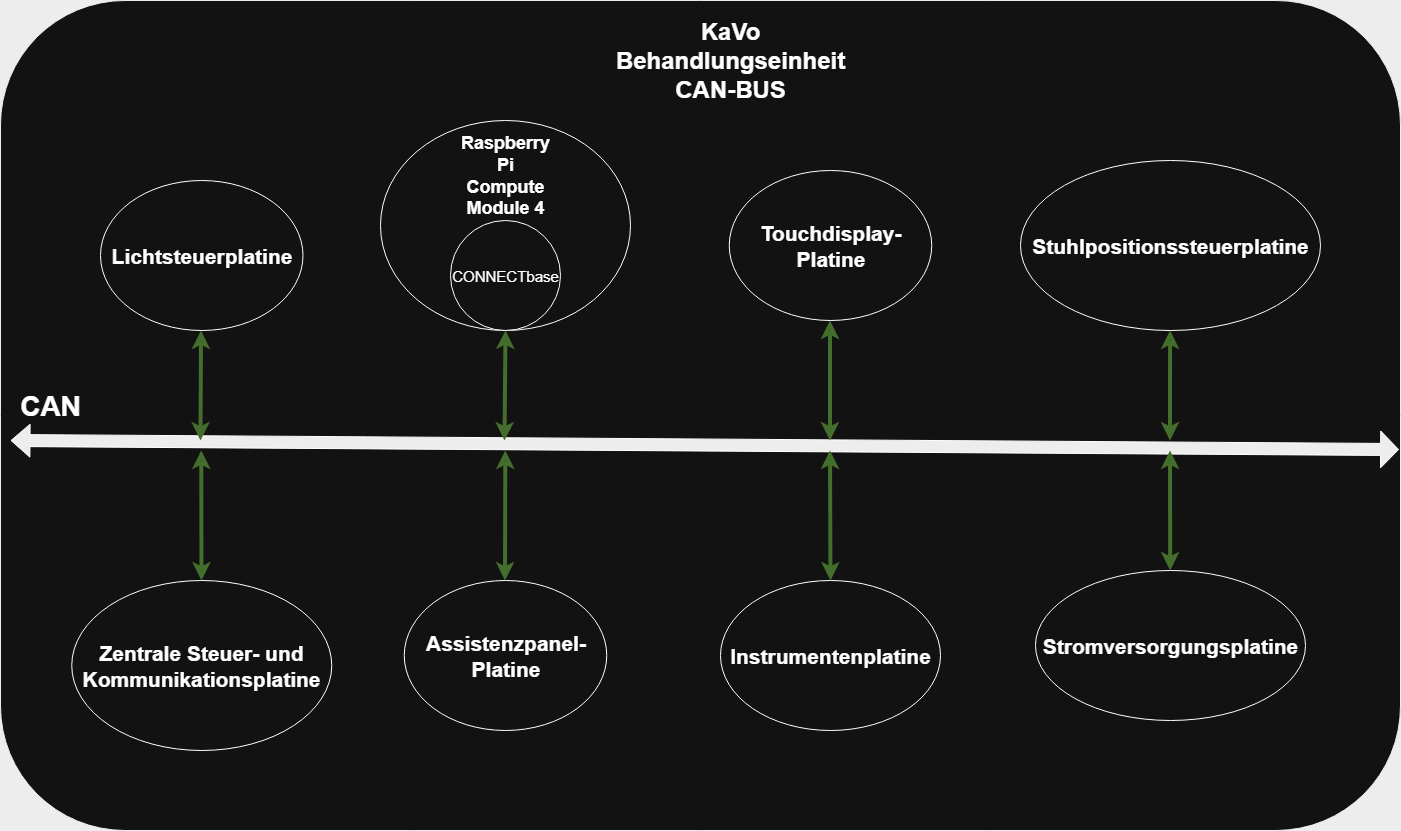
\includegraphics[width=\textwidth]{images/canbus4.drawio.png}
  \end{minipage}
  \hspace{0.05\textwidth}
  \caption{Schematische Darstellung der CAN-Bus-Topologie eines KaVo-Behandlungsstuhls}
  \label{fig:CAN-Bus-Topologie}
\end{figure}
\vspace{1em}

\vspace{1em}
\begin{figure}[H]
  \centering
  \begin{minipage}[b]{1.0\textwidth}
    \centering
    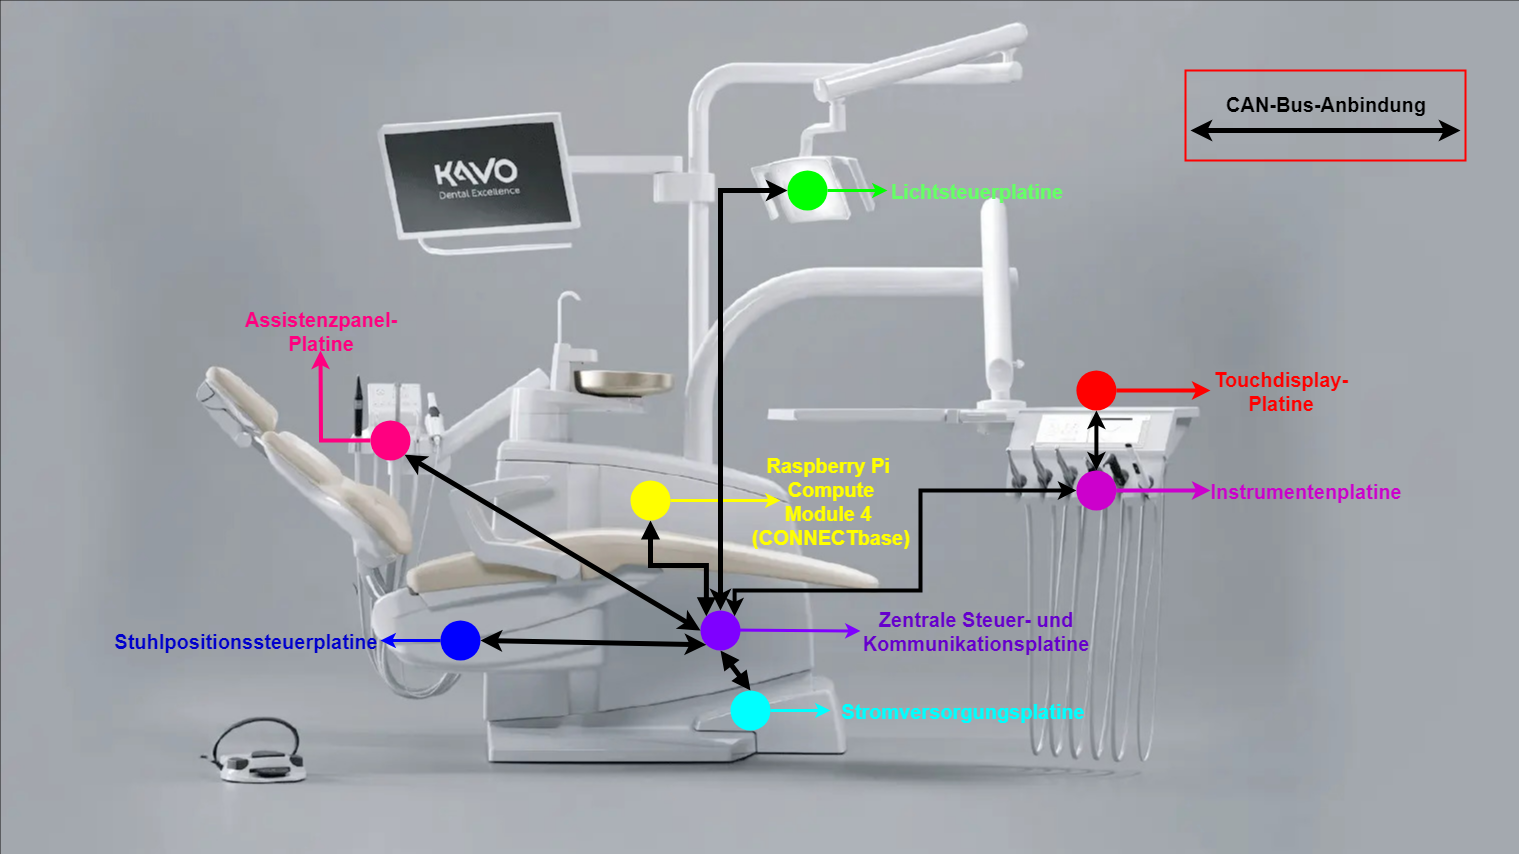
\includegraphics[width=\textwidth]{images/Unbenanntes Diagramm.drawio (4).drawio.png}
  \end{minipage}
  \hspace{0.05\textwidth}
  \caption{Schematische Darstellung der Positionierung der Steuer- und Kommunikationsplatinen im KaVo Behandlungsstuhl mit CAN-Bus-Vernetzung}
  \label{fig:Stuhl_Steuerplatinen_Topologie}
\end{figure}
\vspace{1em}

Diese Architektur reduziert den Verkabelungsaufwand erheblich und unterstützt gleichzeitig eine modulare Erweiterung sowie die einfache Entwicklung neuer Funktionen innerhalb des Behandlungsstuhls.

\subsubsection{Hygieneprogramme und Ablauf in der Praxis}

Zur Aufrechterhaltung höchster Hygienestandards verfügen KaVo-Behandlungsstühle über integrierte Hygieneprogramme, die sich an den Richtlinien des Robert Koch-Instituts orientieren und erfüllen. Diese Programme dienen der automatisierten Spülung und Desinfektion aller wasser- und luftführenden Leitungen sowie der Instrumentenschläuche.

\vspace{1em}
\begin{figure}[H]
  \centering
  \begin{minipage}[b]{0.7\textwidth}
    \centering
    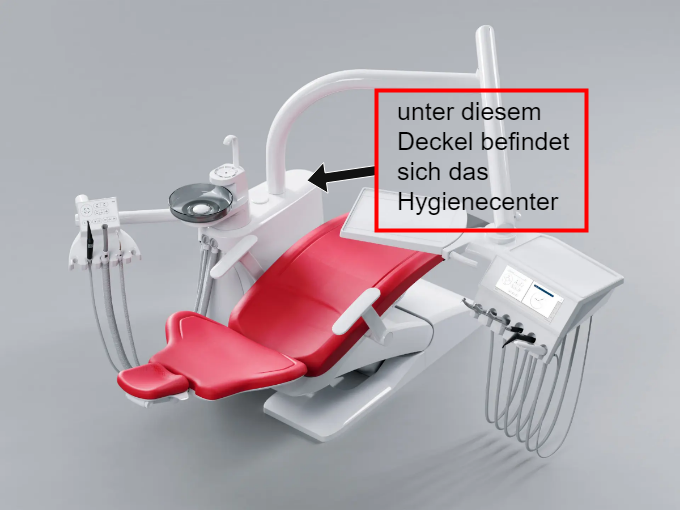
\includegraphics[width=\textwidth]{images/arrowhygienecenter.drawio.png}
  \end{minipage}
  \hspace{0.05\textwidth}
  \caption{Position des Hygienecenters im Behandlungsstuhl.}
  \label{fig:Hygienecenters Position}
\end{figure}
\vspace{1em}

\vspace{1em}
\begin{figure}[H]
  \centering
  \begin{minipage}[b]{0.7\textwidth}
    \centering
    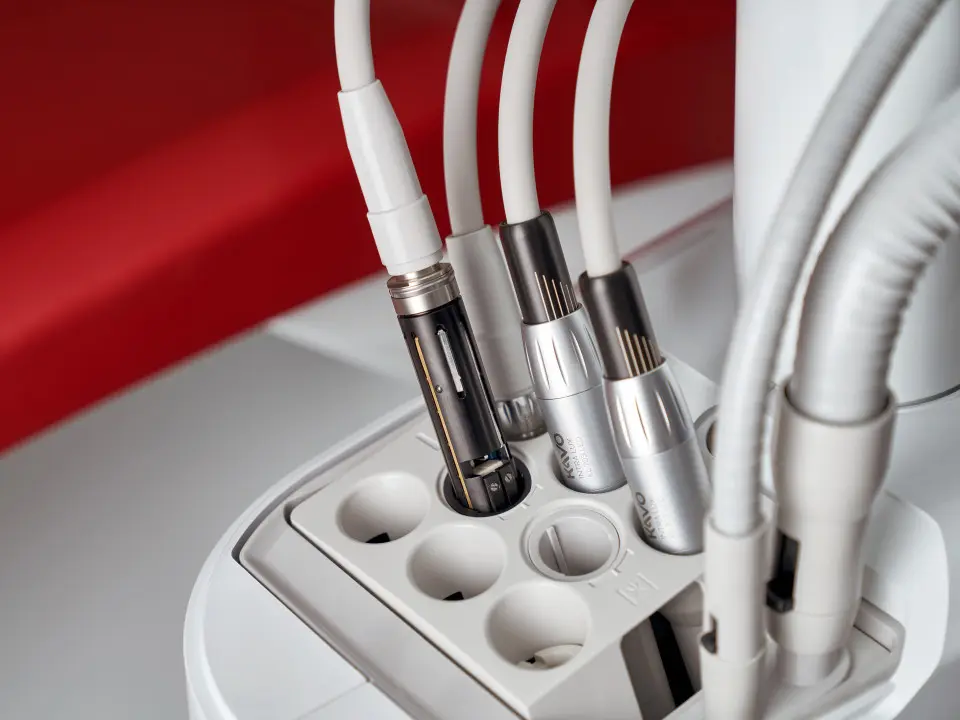
\includegraphics[width=\textwidth]{images/KaVo-uniQa_Hygienecenter_4000px.png}
  \end{minipage}
  \hspace{0.05\textwidth}
  \caption{KaVo Hygienecenter}
  \label{fig:Hygienecenter}
\end{figure}
\vspace{1em}
\newpage
Zentrale physische Schnittstelle dafür ist das sogenannte \textit{Hygienecenter}: eine in den Stuhl integrierte Aufnahme, in der Handinstrumente, Absaugschläuche und Instrumentenschläuche sicher eingehängt werden können. Nach dem Einlegen und starten eines Hygieneprogramms werden die Leitungen automatisch gespült, gereinigt und desinfiziert. Zusätzlich lassen sich Reinigungskartuschen direkt im Hygienecenter einsetzen, die vom System automatisch erkannt und korrekt dosiert werden.

Auf dem Display wird der aktuelle Status angezeigt, einschließlich Restlaufzeit und eventueller Hinweise, sodass eine lückenlose Dokumentation gewährleistet ist.

\vspace{1em}
\begin{figure}[H]
  \centering
  \begin{minipage}[b]{0.7\textwidth}
    \centering
    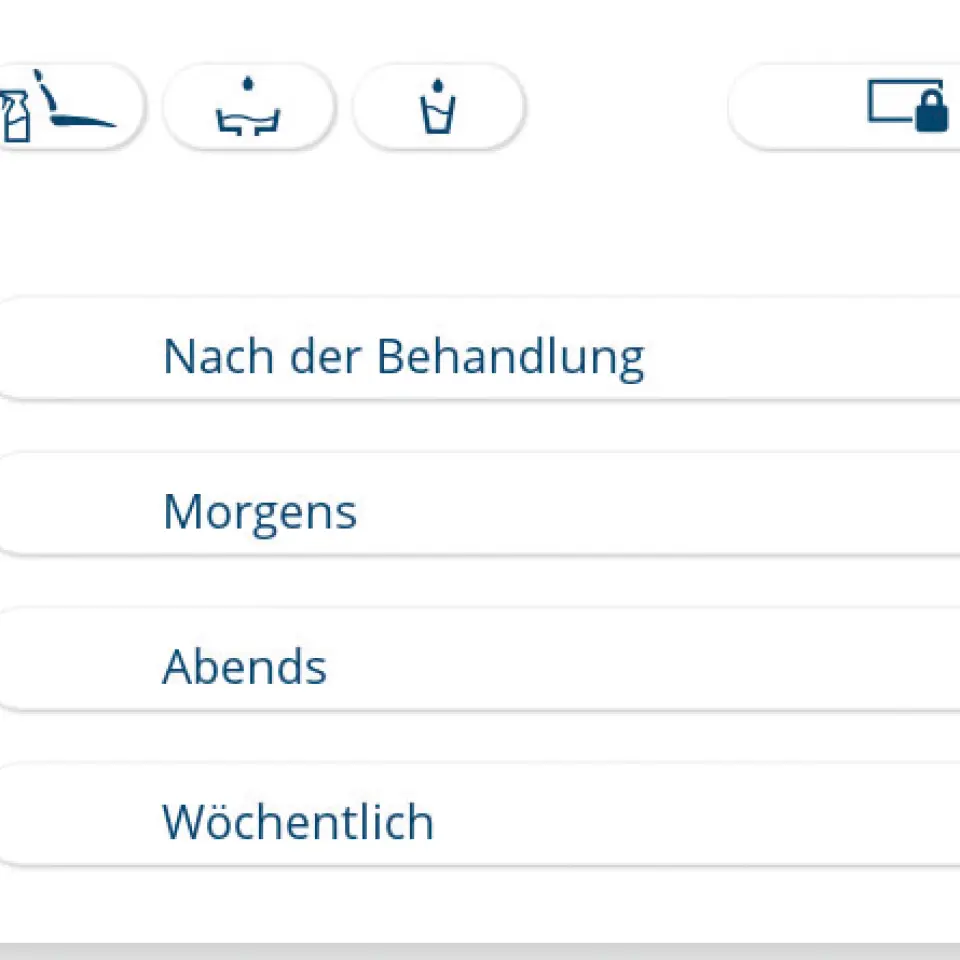
\includegraphics[width=\textwidth]{images/KaVo-amiQa-Display-Behandlung_de.png}
  \end{minipage}
  \hspace{0.05\textwidth}
  \caption{Auswahlmenü der Hygieneprogramme am Touchdisplay}
  \label{fig: Hygieneprogramme am Touchdisplay}
\end{figure}
\vspace{1em}

Aktuell werden verschiedene Hygienezyklen über das Touchdisplay durch das Assistenzpersonal gestartet — zum Beispiel vor Behandlungsbeginn (morgens), nach jedem Patienten (bei Bedarf) und am Abend zur Endreinigung. Diese Abläufe sind in jeder Zahnarztpraxis Standardpraxis und müssen zuverlässig mehrfach täglich wiederholt werden, um eine normgerechte Desinfektion sicherzustellen. Gerade hier bietet sich Potenzial für Automatisierung, um wiederkehrende manuelle Handgriffe zu reduzieren und gleichzeitig die Einhaltung der Hygienerichtlinien zu unterstützen.

Die Ausführung dieser Hygieneprogramme erfolgt vollständig innerhalb der Zentrale Steuer- und Kommunikationsplatine; eine darüber hinausgehende externe Steuerung von Folgeaktionen (z.B. automatisches Abschalten der Stromversorgung nach Abschluss) ist bisher nicht vorgesehen und wird in dieser Arbeit prototypisch realisiert.

\subsubsection{Technischer Ist-Zustand und Marktanforderungen zur Automatisierung}
\label{sec:aktueller-stand-und-automatisierungsanforderung}
Obwohl KaVo-Dentaleinheiten über umfangreiche interne Steuerungs- und Hygieneprozesse verfügen, bestehen funktionale Grenzen: Es gibt keine integrierte Lösung zur intelligenten Stromabschaltung nach Abschluss eines Hygieneplans. Zudem existiert keine standardisierte Möglichkeit, Stuhldaten lokal in Echtzeit an externe Systeme zu übergeben.

Derzeit erfolgt das Ein- und Ausschalten der Dentaleinheit ausschließlich manuell über einen physikalischen Hauptschalter, der sich meist in der Nähe des Behandlungsplatzes befindet. Eine Fernsteuerung oder automatisierte Abschaltung – etwa zur Energieeinsparung oder im Rahmen von Hygieneroutinen – ist nicht vorgesehen. Dieses Vorgehen ist nicht nur umständlich, sondern birgt auch das Risiko, dass der Stuhl nach dem Praxisbetrieb versehentlich eingeschaltet bleibt.

Diese Einschränkungen eröffnen Potenzial für weitergehende Automatisierungen. Insbesondere eine externe, automatisierte Steuerung von Folgeaktionen, wie das Abschalten der Stromversorgung nach Abschluss eines Hygieneplans, könnte dazu beitragen, wiederkehrende manuelle Aufgaben zu reduzieren, Energie zu sparen und die Betriebseffizienz in der Zahnarztpraxis zu erhöhen.

Weitere Details zu diesen Herausforderungen und Anforderungen finden sich im folgenden Kapitel \ref{chap:projektkontext}.

\subsection{CONNECTbase}

\textit{CONNECTbase} ist eine in die KaVo-Dentaleinheit integrierte Komplettlösung aus Hard- und Software, die primär zur Anzeige, Verwaltung und Echtzeit-Darstellung von Bild- und Videodaten während der Behandlung entwickelt wurde. Die zugrunde liegende Hardware basiert auf einem \textit{Raspberry Pi Compute Module 4}, das unter Linux betrieben wird und die Ausführung sowohl einer nativen Oberfläche als auch einer webbasierten Benutzeroberfläche ermöglicht.

Die zentrale Funktionalität von \textit{CONNECTbase} liegt in der nativen C++-Anwendung, die direkt auf dem Hauptbildschirm der Dentaleinheit ausgeführt wird. Sie zeigt unter anderem Livebilder von intraoralen Kameras — wie beispielsweise der \textit{DIAGNOcam Vision Full HD} — an. Alle Inhalte, die auf dem Hauptbildschirm erscheinen, stammen ausschließlich aus dieser nativen Anwendung.

Ergänzend dazu bietet \textit{CONNECTbase} eine Web-GUI, die über das separate Touchdisplay der Einheit bedient wird. Diese Benutzeroberfläche ermöglicht dem Nutzer die Auswahl verschiedener Darstellungsmodi (z.\,B. Patientenbilder oder Livekamera) sowie den Zugriff auf zentrale Einstellungen der Software, wie etwa die Netzwerkkonfiguration, das Hintergrundbild oder das Datenmanagement.

Der unmittelbare Vorgänger von \textit{CONNECTbase} war ein separates analoges Kameramodul in Form einer externen Hardwarebox. Dieses ermöglichte lediglich die Live-Übertragung von Kamerabildern und das Speichern von maximal sechs Bildern. Mit \textit{CONNECTbase} wurden diese Einschränkungen vollständig überwunden. Die neue Systemarchitektur erlaubt eine deutlich umfangreichere Bilddokumentation, eine höhere Rechenleistung und eine stabile Einbindung der Dentaleinheit in ein Netzwerk.

\subsubsection*{Anwendungsbeispiel: Patientenkommunikation in Echtzeit}

Ein typisches Beispielszenario dafür, wie \textit{CONNECTbase} eine effiziente Patientenkommunikation unterstützt, ergibt sich im Umgang mit der intraoralen Kameraeinheit. Wird diese aus ihrer Halterung entnommen, erkennt die Dentaleinheit dies automatisch und versetzt das System in den Live-Modus. Das aktuelle Kamerabild wird dann in Echtzeit auf dem Hauptbildschirm angezeigt. Auf diese Weise kann der Zahnarzt dem Patienten problematische Bereiche unmittelbar visuell erläutern — vergleichbar mit der Benutzerführung moderner Kameraanwendungen.

\subsubsection{Hardwareplattform und Entwicklungsumgebung}

Die Software \textit{CONNECTbase} läuft auf einem \textit{Raspberry Pi Compute Module 4} (CM4), das als kompakte, leistungsfähige Embedded-Hardware innerhalb des KaVo-Behandlungsstuhls eingesetzt wird. Das Compute Module 4 basiert technisch auf dem Raspberry Pi 4 Model B, wurde jedoch speziell für industrielle OEM-Anwendungen konzipiert. Es bietet eine platzsparende Bauform, flexible Speicherkonfigurationen (eMMC-Flash oder microSD) sowie erweiterte Anschlussmöglichkeiten über ein maßgeschneidertes Carrier-Board.

\begin{figure}[H]
  \centering
  \begin{minipage}[b]{0.45\textwidth}
    \centering
    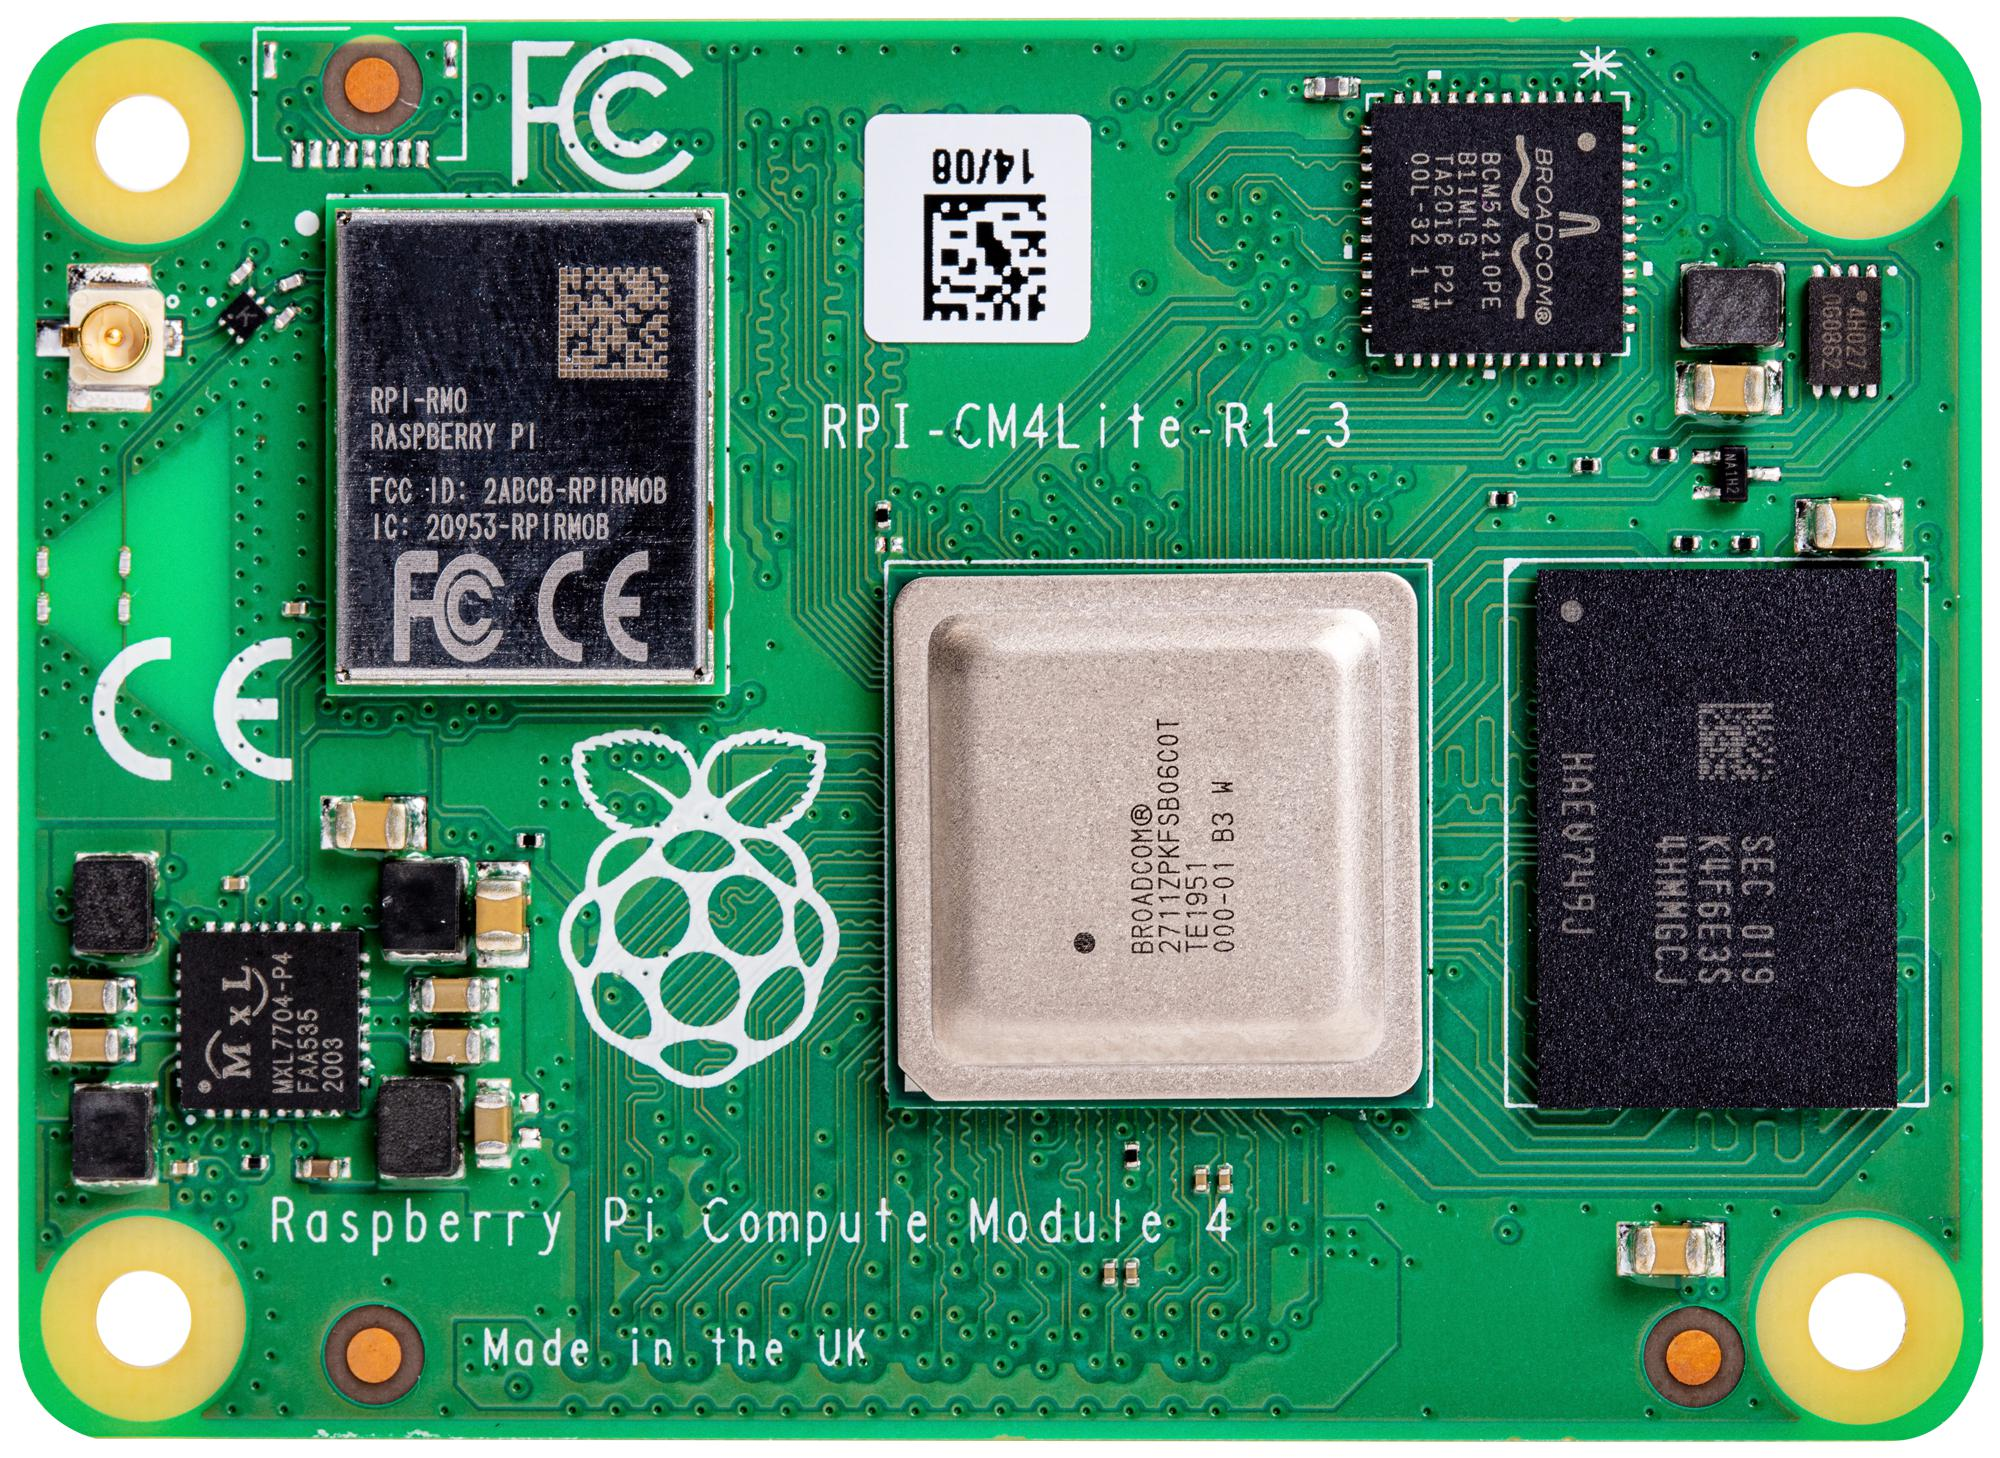
\includegraphics[width=\textwidth]{images/computemodule4.jpg}
    \caption*{Raspberry Pi Compute Module 4}
  \end{minipage}
  \hspace{0.05\textwidth}
  \begin{minipage}[b]{0.45\textwidth}
    \centering
    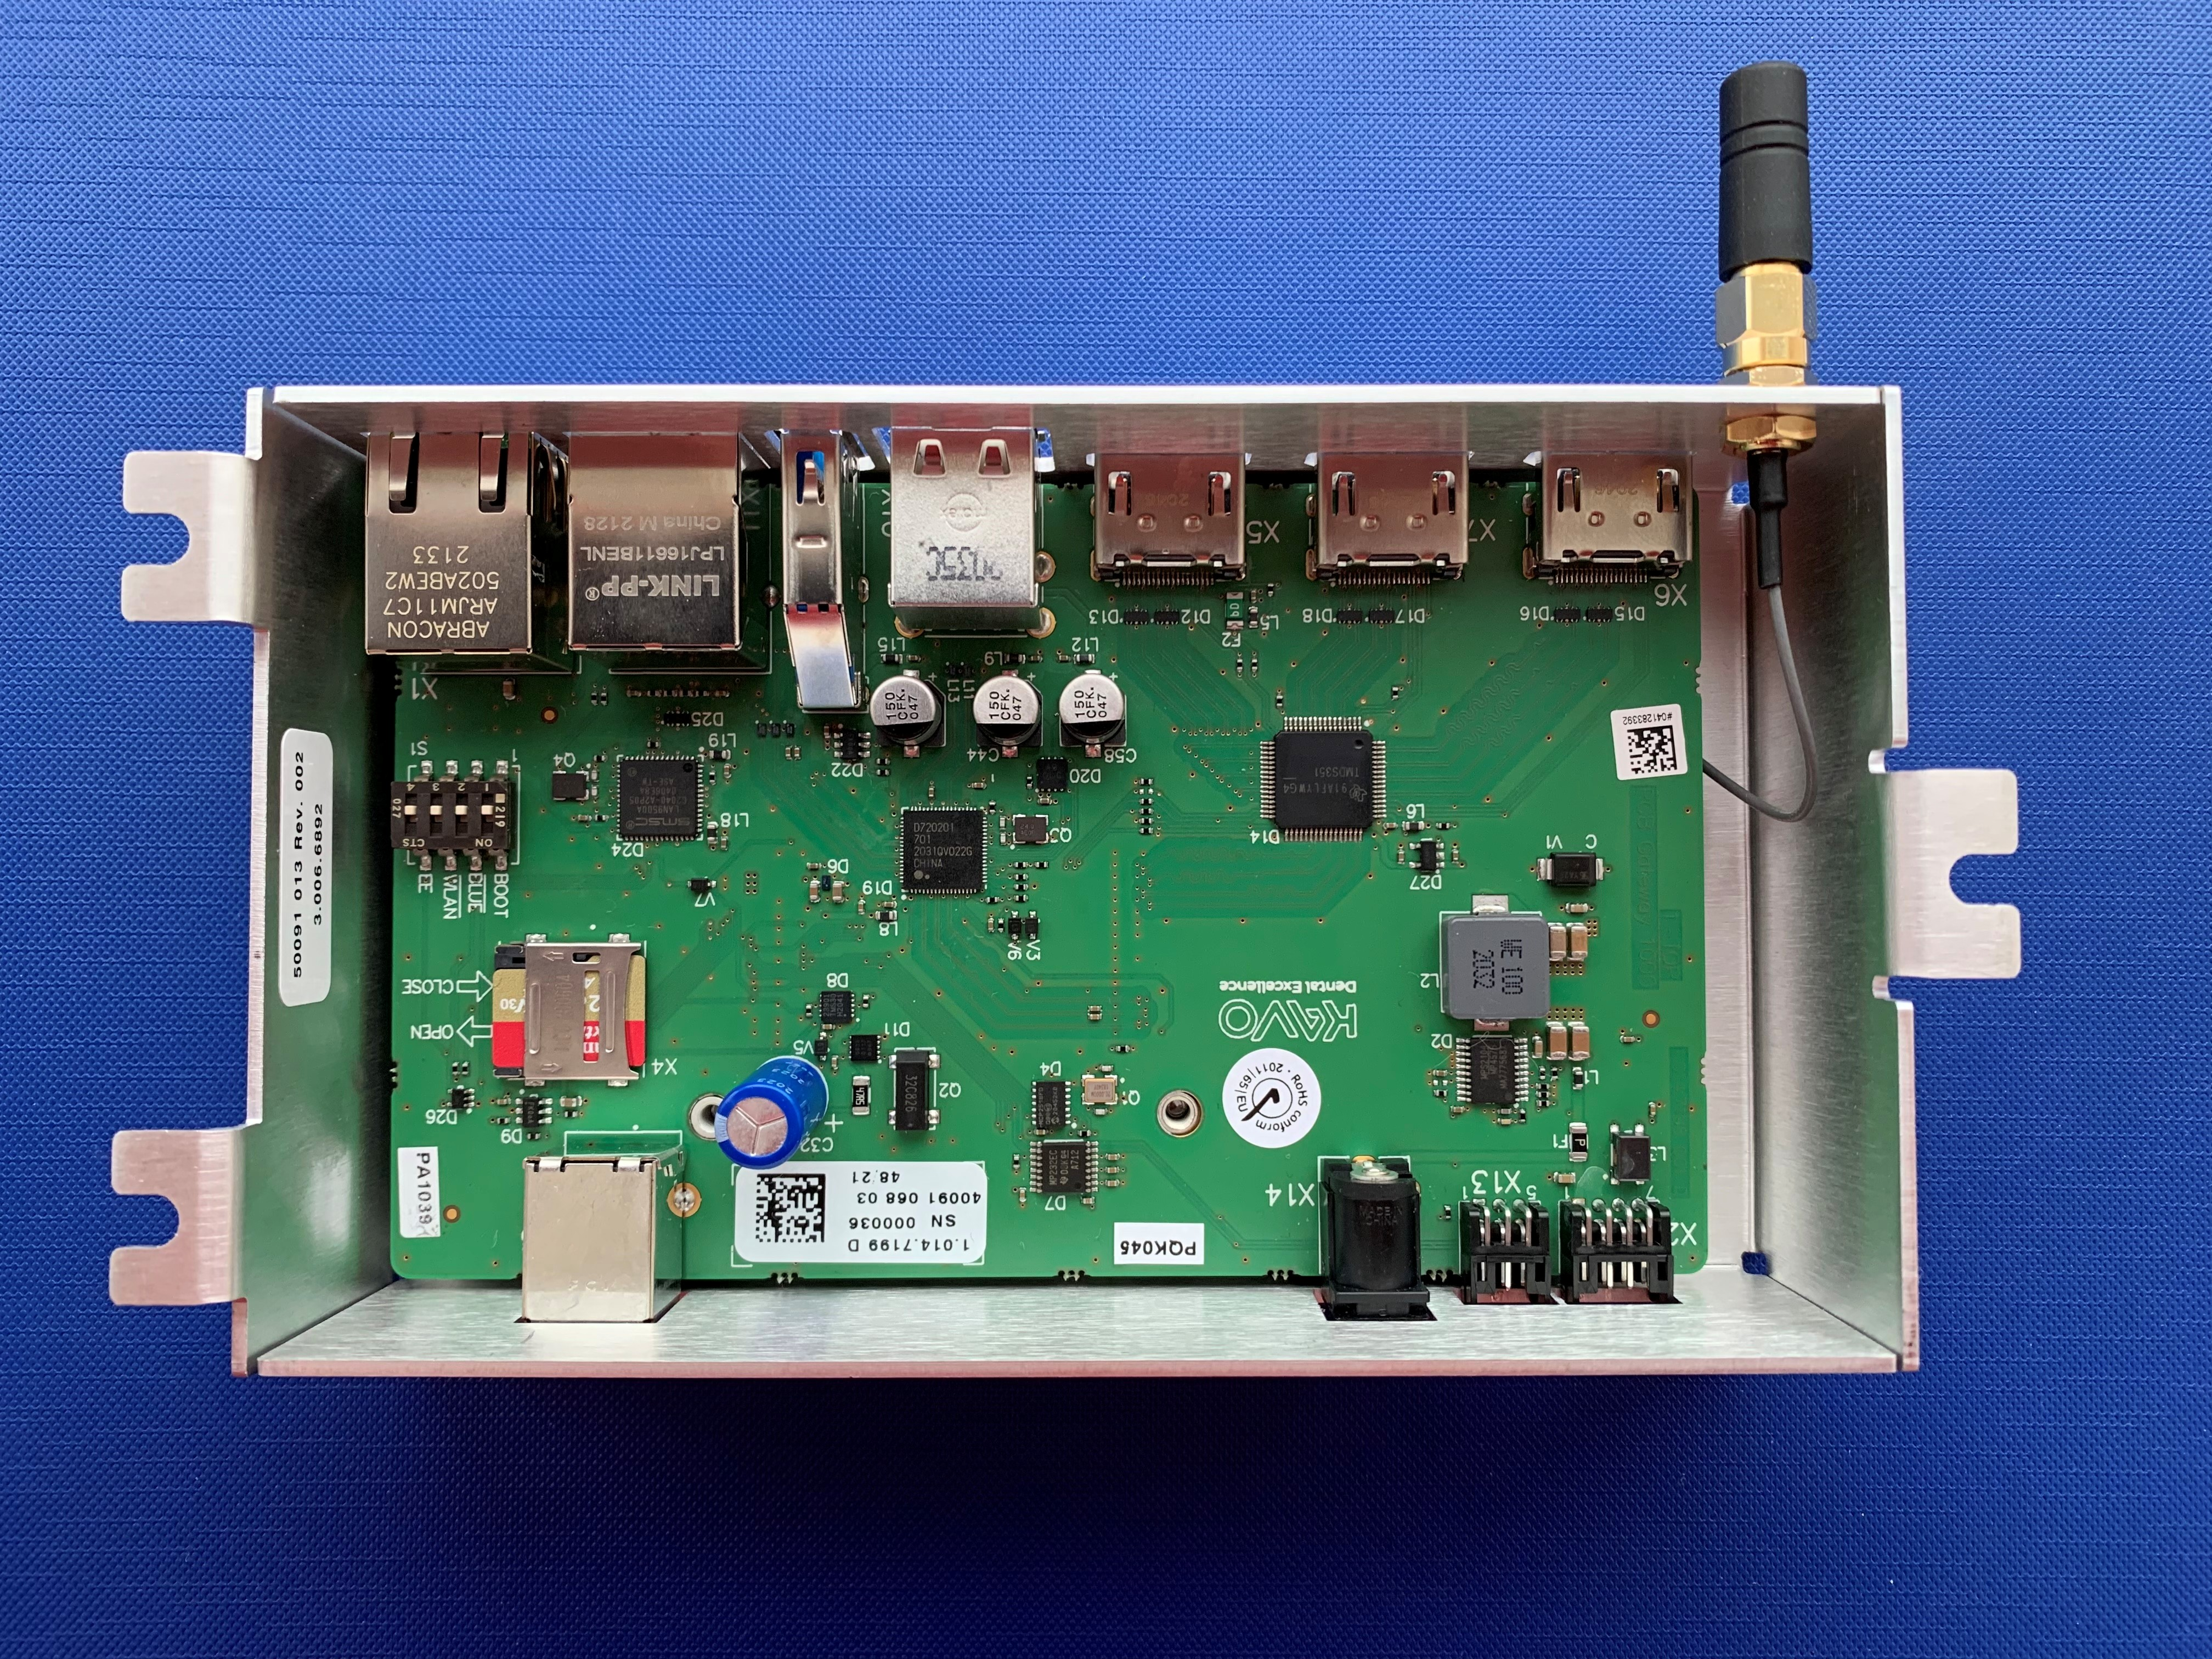
\includegraphics[width=\textwidth]{images/carrierboard.jpg}
    \caption*{KaVo Carrier-Board}
  \end{minipage}
  \caption{KaVo CONNECTbase Hardware}
  \label{fig:CONNECTbase Hardware}
\end{figure}
\vspace{1em}
Im KaVo-System übernimmt das CM4 die Rolle eines eigenständigen Mitglieds im internen \textit{CAN-Bus}-Netzwerk. Es steuert keine Kernfunktionen des Stuhls wie Motorbewegungen oder Instrumente direkt, sondern ist ausschließlich für die Erfassung, Verarbeitung und Anzeige von Bild- und Videodaten zuständig. Über den CAN-Bus tauscht es Statusinformationen aus und kann bei Bedarf Daten an andere Systeme weitergeben oder empfangen.

\begin{figure}[H]
  \centering
  \begin{minipage}[b]{0.82\textwidth}
    \centering
    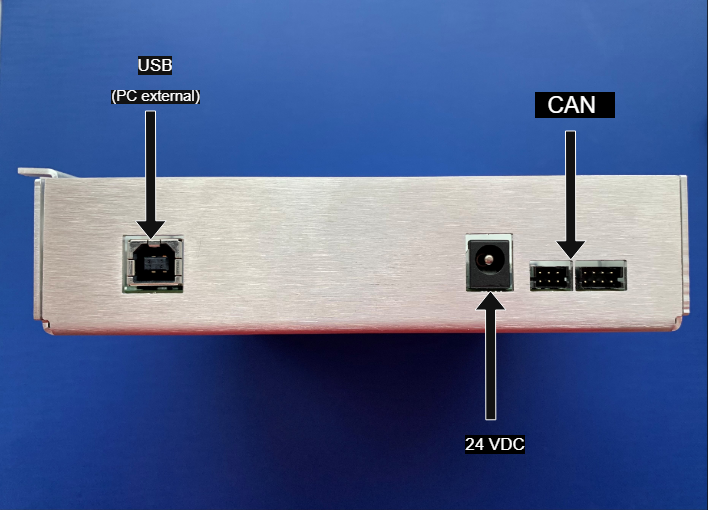
\includegraphics[width=\textwidth]{images/canfixed.drawio.png}
  \end{minipage}
  \hspace{0.05\textwidth}
  \caption{Rückseite des speziell entwickelten Carrier-Boards}
  \label{fig:CarrierBoardRueckseite}
\end{figure}
\vspace{1em}

Das Carrier-Board im Stuhl ist speziell an die Anforderungen angepasst: Es stellt mehrere HDMI-Eingänge und ein HDMI Ausgang für den Bildschirm des Behandlungsstuhls bereit, diverse USB-Ports (für Kameras oder Servicezugänge), Dual-LAN-Anbindungen sowie CAN-Schnittstellen. Diese Hardware-Integration ermöglicht es, Bildsignale in hoher Auflösung zu verarbeiten, Live-Streams anzuzeigen und gespeicherte Aufnahmen effizient zu verwalten.

\begin{figure}[H]
  \centering
  \begin{minipage}[b]{0.82\textwidth}
    \centering
    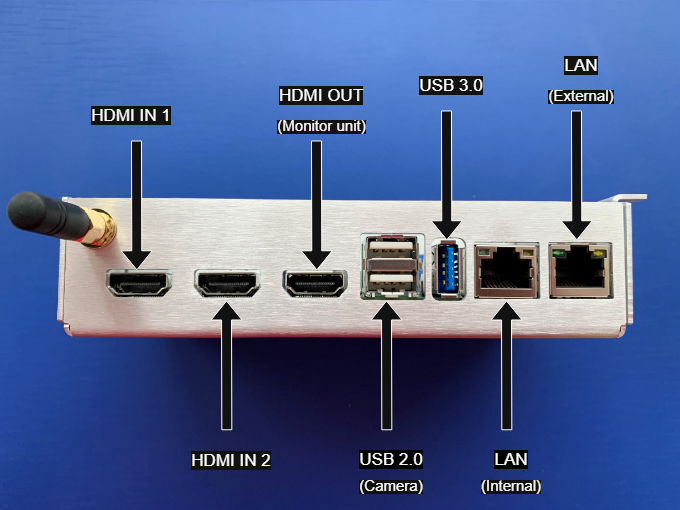
\includegraphics[width=\textwidth]{images/connectbaseport2.drawio.png}
  \end{minipage}
  \hspace{0.05\textwidth}
  \caption{Vorderseite des speziell entwickelten Carrier-Boards}
  \label{fig:CarrierBoardVorderseite}
\end{figure}
\vspace{1em}

Die Software von \textit{CONNECTbase} selbst wurde in \textit{C++} entwickelt und nutzt das plattformübergreifende \textit{Qt}-Framework für die Benutzeroberfläche und das Event-Handling. Entwickelt und gewartet wird die Lösung mit \textit{Qt Creator}, was eine modulare Codebasis und einfache Erweiterbarkeit unterstützt.

Die Kombination aus Compute Module 4 und Qt-basierter Softwarearchitektur erlaubt KaVo, mit begrenztem Platz- und Energiebedarf eine robuste, flexible und langfristig wartbare Plattform für Bilddokumentation und vernetzte Funktionen im Stuhl bereitzustellen.
